

\section{Motivation}

In an afternoon of 2017, humanity had an unlikely champion. Ke Jie, the number one player in GO, was to battle against one of the world's most intelligent machines, AlphaGo; a powerhouse of artificial intelligence backed by one of the world's top technology company: Google. Since the number of possible positions on a Go board exceeds the quantity of atoms in the universe, defeating the world champion was the biggest deed possible for AI researchers at the time. Romantics said it was impossible for a machine to do so as it lacked spiritual power only a human could possess, engineers would agree but by a different reason, they pointed out for the fact that there was just too many possibilities for a computer to evaluate; these ``theories'' fell apart though. On this day, what was witnessed was not a clash between two equal titans, AlphaGo  completely dominated Ke Jie. Over the course of three marathon matches of more than three hours each, the top ranked player tried every single approach: conservative, aggressive, defensive and unpredictable. Nothing worked, there were no openings, not a single sign of hope.

\begin{figure}[h]
	\centering
	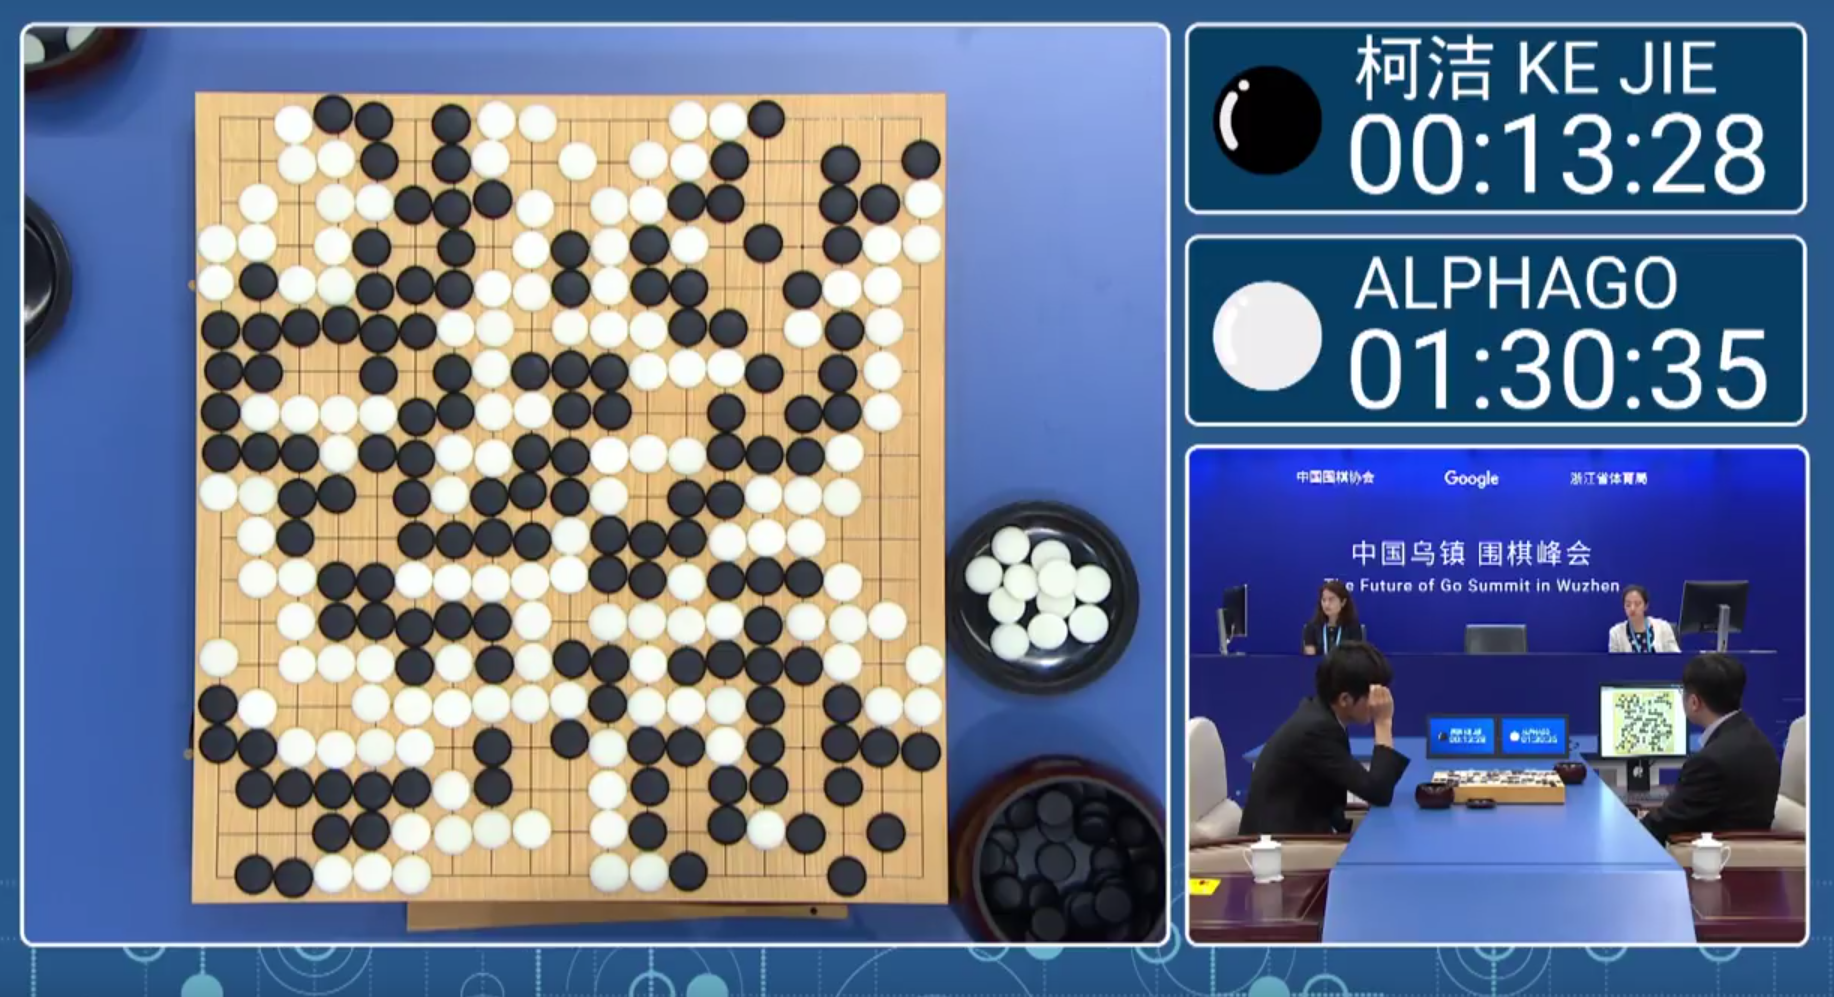
\includegraphics[width=1.0\textwidth]{Cap1/AlphaGo1.png}
	\caption{Ke Jie faces AlphaGo}
	\label{AlphaGo1}
\end{figure}

\begin{figure}[h]
	\centering
	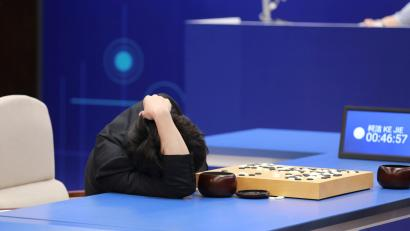
\includegraphics[width=1.0\textwidth]{Cap1/AlphaGo2}
	\caption{Ke Jie is ultimately defeated}
	\label{AlphaGo2}
\end{figure}

\subsection{AI Super Powers}

As described by \cite{AISuperPowers2018}, this event is the equivalent of Sputnik for China. Less than two months after Ke Jie resigned his last game to AlphaGo, the central government of China issued an ambitious plan to build artificial intelligence capabilities. China designed a clear strategy, set benchmarks for progress by 2020 and 2025 aiming to be the center of global innovation in artificial intelligence. Private money answered that call, Chinese venture-capital investors had already responded to that call, unleashing record amounts into AI startups and making up 48 percent of all AI venture funding globally, surpassing the United States for the first time.

Less than two months after Ke Jie resigned his last game to AlphaGo, the Chinese central government issued an ambitious plan to build artificial intelligence capabilities. It called for greater funding, policy support, and national coordination for AI development. It set clear benchmarks for progress by 2020 and 2025, projected that by 2030 China would become the center of global innovation in artificial intelligence, leading in theory, technology, and application. By 2017, Chinese venture-capital investors had already responded to that call, pouring record sums into artificial intelligence startups and making up 48 percent of all AI venture funding globally, surpassing the United States for the first time.

The fact that the current global economic power and the one aspiring to be  are massively investing on AI technology points at first hand that the topic is worth studying for. The State of AI in the Enterprise 2nd Edition conducted by Deloitte \cite{AiSurvey} gives some numbers on how AI is making the industry grow: ``To obtain a cross-industry view of how organizations are adopting and benefiting from cognitive computing/AI, Deloitte surveyed 1,100 IT and line-of-business executives from US-based companies in Q3 2018. All respondents were required to be knowledgeable about their company's use of cognitive technologies/artificial intelligence, and 90 percent have direct involvement with their company's AI strategy.''. According to it, 82 per cent of the survey participants claim a positive financial return on their AI investment and 88 per cent plan to increase spending in 2019; 79 per cent agree that AI technologies empower people to make better decisions and 73 per cent believe AI will increase job satisfaction. Furthermore, the graphic \ref{Deloitte} shows that around 75 per cent reported positive results when comparison to direct competitors was made.

\begin{figure}[h]
	\centering
	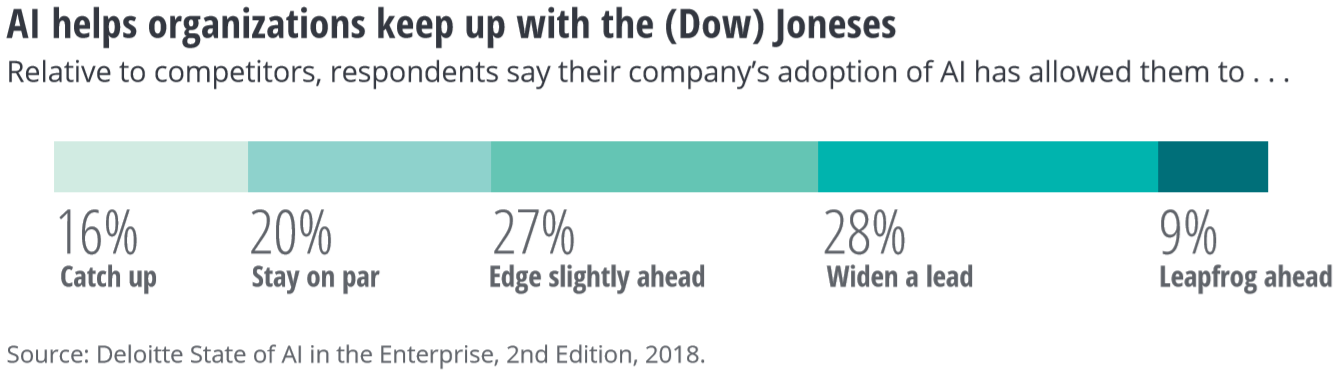
\includegraphics[width=1.0\textwidth]{Cap1/AI_Deloitte}
	\caption{Distribution of answers of  1,100 candidates from Deloitte's survey about AI in the Enterprise on how the technology levered their business production in comparison to their competitors}
	\label{Deloitte}
\end{figure}

What are the results AI can bring to justify this current fever? \cite{PredictionMachines2018} puts it simply, AI is a technology that optimizes and facilitates decisions and predictions. For example, the article \cite{FacialRec} talks about the Shanghai-based YITU Technology that  has gained wide recognition for its Dragonfly Eye System, a facial scanning platform that can identify a person from a database of at least 2 billion people in a matter of seconds .\cite{Zymergen} talks about  Zymergen, a company that uses machine learning to navigate the genomic search space in order to guide scientists to the precise set of genetic changes required to engineer cells to make a product of interest or to do it more efficiently. The applications are too numerous to cite them all but these two examples represent how broad the technology can go and how the future is being passed by it. The graphic \ref{Deloitte2} is from \cite{AiSurvey} and it shows more specifically how AI generate 

\begin{figure}[h]
	\centering
	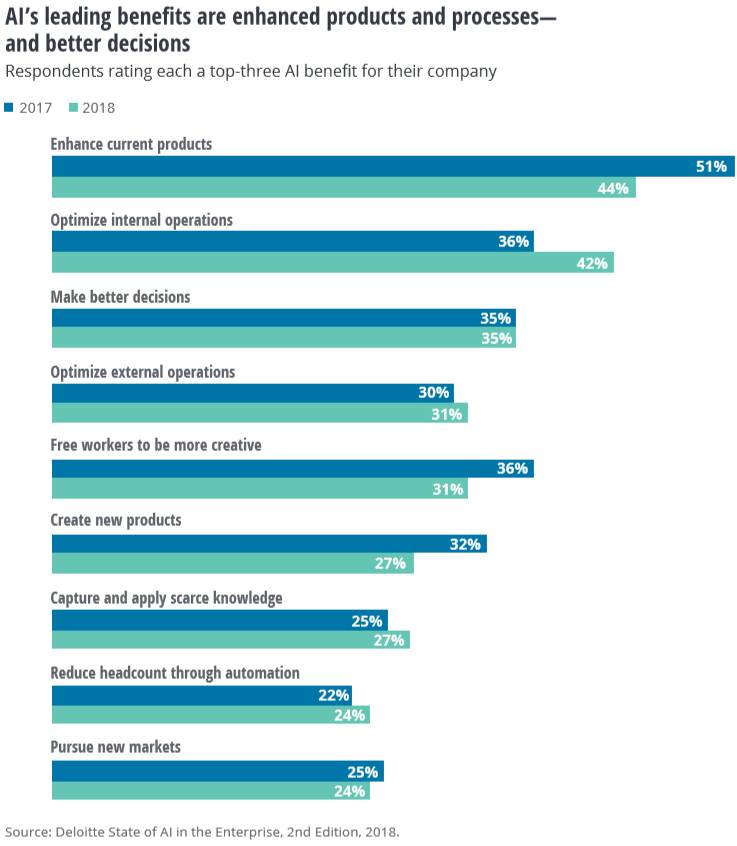
\includegraphics[width=1.0\textwidth]{Cap1/AI_Deloitte2}
	\caption{How AI brings benefit according to the surveyed candidates from Deloitte report}
	\label{Deloitte2}
\end{figure}

\subsection{Deep Learning Revolution}

Machine learning , despite being this new driver of the future, is lucky to have survived a tumultuous half-century of research. For each great promising new lead there were big voids too, when weak practical results led to investments retraction.

There were 2 camps in the field: the ``rule-based'' approach and the ``neural networks'' approach. Researchers of the first attempted to teach computers to think by encoding a series of logical rules (If Then and Else). This method worked well for simple and well defined problems for example a game of Sudoku but when the universe of options was too large it did not respond well. Their insight was too question experts on the problem at hand and try to embody their wisdom into the machine (Hence why this method is also called the ``expert systems'').

The ``neural network'' approach goes a different route by trying to reconstruct the brain itself, taking inspiration on the one and only source of intelligence we could perceive. This approach mimics the neurological architecture of the biological brain and instead of trying to transfer knowledge by force like the first one, this approach just feeds the neural networks with a plenitude of data and lets it find patterns on it.

\cite{AISuperPowers2018} gives a simple illustration on how the techniques differ, if it is desired for the computer to recognize the picture of a cat, the ``rule based'' approach would work by trying, for starters, to embed the machine with the idea that a cat has 2 triangles above a circle. In the ``neural network'' approach, the machine would be fed with tones of pictures of cats and non-cats for it to build the features of what is a cat on its own.

To make things short, promising results were achieved during 1950s and 1960 by artificial neural networks but its core methodology found 2 problems that could not be solved at the time, first it needed a lot of data and second a lot of computational power. It quickly went out of fashion then and AI entered into one of its first ``winters'' during the 1970s.

It was not just the increased computing force that came with time which reanimated neural networks, a huge chunk of credit must be given to the optimization in the algorithm itself discovered by leading researcher Geoffrey Hinton and his Convolution Neural Networks (CITAR PAPER ORIGINAL). This new empowered neural network-now re-branded as ``deep learning''- could outperform older models at a variety of tasks. However, the real demonstration occurred in 2012, when a neural network built by Hinton's team overpowered the competition in an international computer vision contest.

\subsection{Reinforcement Learning}
Although companies have been using AI, they are mostly using them to make predictions as written in \cite{PredictionMachines2018}, in other words, they do things like predict which product a costumer might want given an history of purchases or which size of clothing best suits the client. These are not necessarily and often not done  by Reinforcement Learning(A branch of Machine Learning), which is the precise topic of this thesis. 

Although still not fully incorporated into corporations, Reinforcement Learning is not to be neglected for it is paving the road of more powerful innovations, here are some recent papers showing the technique applications.
\
\begin{itemize}
	\item{\textbf{Resources Management in Computer Clusters}}: The paper \cite{Resource} Learning)  showed how to use RL to automatically learn to allocate and schedule computer resources to waiting jobs, with the objective to minimize the average job slowdown.
	\item \textbf{Traffic Signal Control }In the paper \cite{Traffic}, researchers built a traffic light controller to solve congestions problems. In simulations, their methods showed great improvement from the state-of-art techniques; they also accomplished decent results in real scenarios.
	\item \textbf{Optimizing Chemical Reactions} In the paper \cite{Chemistry}, researchers built a mode that iteratively records the results of a chemical reaction and chooses new experimental conditions to improve the reaction outcome. outperforming a state-of-the-art black box optimization algorithm by using 71\% fewer steps on both simulations and real reactions. 
\end{itemize}

\section{Contextualization}

RoboCup is an international scientific community aiming to advance the state of the art of intelligent robots. Its mission is that a team of androids will be able to beat the human team champion of the World Cup until the year 2050 \cite{RoboCup}. To achieve this goal, there is actually a plenitude of tasks to be solved, if you actually enumerate what a professional player must know, the difficulty stacks up. 

For example, to kick a ball, a thing we humans almost take for granted, there is a complex mixture of muscle movements and positioning that a robot would have to mimic. Of course when you think about soccer you think about kicking but there is way more: to carry the ball a certain distance, to pass, to tackle, to receive a pass; these are all complex set of movements that requires good hardware and software coordination.

Soccer is not a pure athletic sport though, that means victory is not only decided by being more able, stronger or faster. It is a versus sport, the players must decide how to act in different conditions, when to run, where to position themselves and what movement to make according to the enemy same actions.

\subsection{Simulated Soccer 2D}
Directly from the RoboCup official site \cite{RoboCup}: ``In the 2D Simulation League, two teams of eleven autonomous software programs (called agents) each play soccer in a two-dimensional virtual soccer stadium represented by a central server, called SoccerServer. This server knows everything about the game, i.e. the current position of all players and the ball, the physics and so on. The game further relies on the communication between the server and each agent. On the one hand each player receives relative and noisy input of his virtual sensors (visual, acoustic and physical) and may on the other hand perform some basic commands (like dashing, turning or kicking) in order to influence its environment.''

In other words, this category focus on the behavior of a soccer player and disregard body-physics implementations.

\begin{figure}[h]
	\centering
	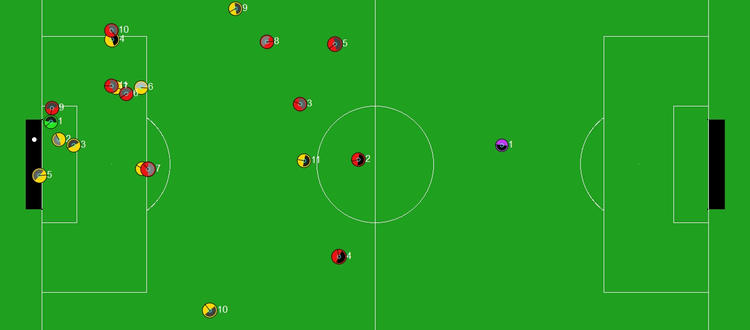
\includegraphics[width=0.7\textwidth]{Cap1/Soccer2D}
	\caption{Simulated Soccer 2D League}
	\label{Soccer2D}
\end{figure}

\section{Objective}
The objective of this bachelor's thesis is to use Deep Learning in order to optimize  the behavior of the goalkeeper  agent in Simulated Soccer 2D, under the more constricted penalty scenario in which the goalkeeper faces in a one-on-one dispute against  an attacker  that starts with  the ball and is fairly distanced from the goalkeeper whose initial position lies in the goal area. Currently, unlike real soccer game, the rules accept that the goalkeeper can move freely during the penalty.

\section{Scope}
The scope of this work is Reinforcement Learning, to use  \textit{Actor-Critic Method} with \textit{PPO}(Proximal Policy Optimization). 

\section{Organization of this work}
\begin{itemize}
	\item On chapter 2 a brief overview of the soccer 2D and the task at hand is made.
	\item On chapter 3 the theory of Deep Learning is presented.
	\item On chapter 4 a plan of execution is scheduled.
\end{itemize}






















